\documentclass[twocolumn, fontsize=10pt]{article}

\raggedbottom
\setlength{\parskip}{0pt}

\usepackage[margin=0.80in]{geometry}
\usepackage{lipsum,mwe,abstract}
\usepackage[T1]{fontenc}
\usepackage[english]{babel}
\usepackage{fancyhdr}
\pagestyle{fancyplain}
\fancyhead{}
\fancyfoot[C]{\thepage}
\setlength\parindent{0pt}
\usepackage{booktabs,tabularx,caption,hyperref}
\usepackage{natbib}
\usepackage{amsmath,amsfonts,amsthm}
\usepackage{graphicx}
\usepackage{float}
\usepackage{subcaption}
\usepackage{comment}
\usepackage{enumitem}
\usepackage{cuted}
\usepackage{booktabs}
\usepackage{sectsty}
\usepackage{dblfloatfix}
\usepackage{placeins}
\setlength{\dbltextfloatsep}{8pt plus 2pt minus 2pt}
\usepackage{cuted}
\usepackage{capt-of}
\usepackage{graphicx}
\usepackage[dvipsnames]{xcolor}
\usepackage[most]{tcolorbox}
\usepackage{tikz}
\usetikzlibrary{arrows.meta}

% ── Colour palette ────────────────────────────────────────────────────────────
\definecolor{RBlue}{HTML}{2E4A7C}
\definecolor{RBlueLight}{HTML}{90AEC1}
\definecolor{RSand}{HTML}{F2CB80}
\definecolor{RGray}{HTML}{E0E2DC}
\definecolor{CodeBG}{HTML}{F7F8FA}
\definecolor{ElegantNavy}{HTML}{0E2A47}
\definecolor{SteelBlue}{HTML}{4B6E8A}
\definecolor{DeepGrey}{HTML}{333333}
\definecolor{RCharcoal}{HTML}{2B2B2B}
% Legend colours
\definecolor{SKBlue}{HTML}{4472C4}
\definecolor{SKOrange}{HTML}{E6A020}
\definecolor{SKRed}{HTML}{C0392B}
\definecolor{SKGreen}{HTML}{2E8B57}
\definecolor{SKPurple}{HTML}{7B2D8B}
\definecolor{SKGray}{HTML}{595959}
\definecolor{SKNavy}{HTML}{2E4A7C}
\definecolor{LegBG}{HTML}{F7F8FA}
% Caption colourboxes
\definecolor{BagOrange}{HTML}{E6A020}
\definecolor{InnerYellow}{HTML}{F5C518}
\definecolor{RedBranch}{HTML}{C0392B}
\definecolor{GreenDeploy}{HTML}{1E8449}

% ── Legend shape macros ───────────────────────────────────────────────────────
\newcommand{\swatch}[1]{\tikz[baseline=-1pt,line width=0.7pt]%
  \draw[fill=#1!25,draw=#1](0,0pt) rectangle (9pt,9pt);}

\newcommand{\Sarrow}[3]{%
  \tikz[baseline=1.5pt,line width=#3]
    \draw[#1,#2,-{Stealth[length=5pt,width=3.5pt]}](0,0)--(1.2cm,0);}

% ── Typography ────────────────────────────────────────────────────────────────
\renewenvironment{abstract}{%
 {\small\begin{center}\bfseries\abstractname\vspace{-.5em}\vspace{0pt}\end{center}
  \list{}{\setlength{\leftmargin}{0mm}\setlength{\rightmargin}{\leftmargin}}
  \item\relax}}{\endlist}

\makeatletter
\renewcommand{\maketitle}{\bgroup\setlength{\parindent}{0pt}
\begin{flushleft}\@title\@author\\\@date\end{flushleft}\egroup}
\makeatother

\hypersetup{colorlinks=true,linkcolor=RBlue,citecolor=blue,urlcolor=RBlue}

\definecolor{captiongray}{gray}{0.35}
\captionsetup[figure]{font=small,labelfont={bf,color=captiongray},textfont={color=captiongray}}
\captionsetup[table]{font=small,labelfont={bf,color=captiongray},textfont={color=captiongray}}
\captionsetup[subfigure]{font=footnotesize,labelfont={bf,color=captiongray},textfont={color=captiongray}}

\sectionfont{\color{ElegantNavy}\bfseries\fontsize{11}{13}\selectfont\MakeUppercase}
\subsectionfont{\color{SteelBlue}\bfseries\fontsize{10}{12}\selectfont}
\subsubsectionfont{\color{DeepGrey}\bfseries\fontsize{9}{11}\selectfont}

% ── Title ─────────────────────────────────────────────────────────────────────
\title{%
  \Large\centering
  \textbf{Intelligible Models for Healthcare: Predicting Pneumonia Risk
          and Hospital 30-day Readmission}\\[6pt]
  \large\textcolor{RCharcoal}{Paper Review, Machine Learning, Assignment 4}\\[10pt]}
\date{\today}
\author{{\normalsize
  Iñigo Arriazu García, Laia Colomé Xicoy, Andrea Pérez Valle,
  Joana Ros Alonso, Gabriel Torres Zamora}}

% ─────────────────────────────────────────────────────────────────────────────
\begin{document}
\twocolumn[\maketitle]

% ─────────────────────────────────────────────────────────────────────────────
\section{Pipeline Diagram}
\label{sec:pipeline}
% ─────────────────────────────────────────────────────────────────────────────

Figure~\ref{fig:pipeline} presents the full ML workflow of
\citet{caruana2015intelligible}, from raw patient data through to clinical
deployment, across three stages: \textbf{(i)}~GAM training via
gradient-boosted shallow trees with bagging; \textbf{(ii)}~GA\textsuperscript{2}M
extension via pairwise interaction detection in the GAM residuals; and
\textbf{(iii)}~expert clinical review with optional model correction before
deployment.


% ─────────────────────────────────────────────────────────────────────────────
\section*{AI Usage}
For this assignment, we used AI tools to help optimise and elaborate our
code and improve the overall structure and flow of the text. All core
decisions, analytical approaches, and the written report content are our
own, based primarily on the class materials and literature.

% ── Bibliography ──────────────────────────────────────────────────────────────
\bibliographystyle{plainnat}
\begin{thebibliography}{99}

\bibitem[Caruana et al.(2015)]{caruana2015intelligible}
Caruana, R., Lou, Y., Gehrke, J., Koch, P., Sturm, M., \& Elhadad, N. (2015).
\newblock Intelligible models for healthcare: Predicting pneumonia risk and
  hospital 30-day readmission.
\newblock In \textit{Proceedings of the 21st ACM SIGKDD International
  Conference on Knowledge Discovery and Data Mining} (pp.\ 1721--1730). ACM.

\end{thebibliography}

% ── Full-page pipeline figure (placed on its own page) ────────────────────────
\begin{figure*}[p]
  \centering

  %% ── Shape key image ────────────────────────────────────────────────────────
  
\includegraphics[width=0.92\linewidth]{shape.png}

  \vspace{6pt}



  \vspace{8pt}

  %% ── Main diagram ───────────────────────────────────────────────────────────
  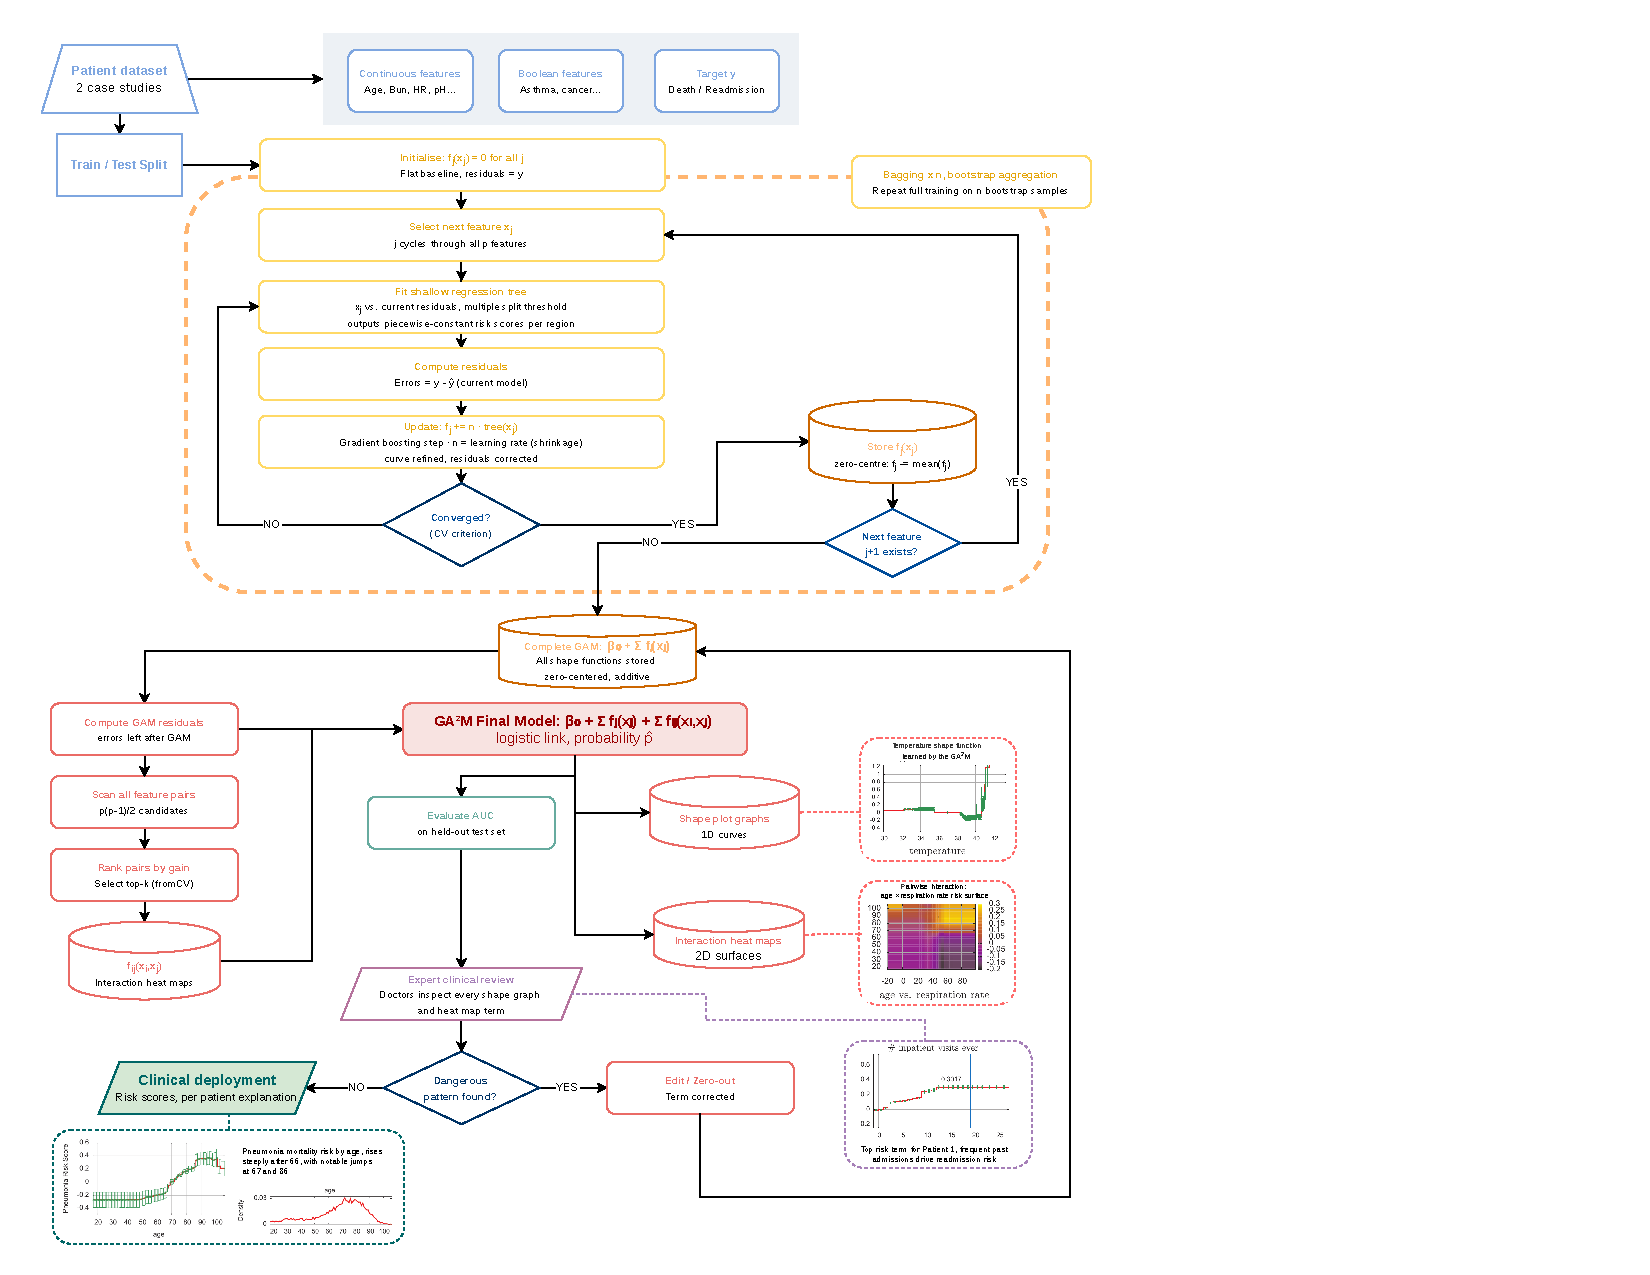
\includegraphics[width=\linewidth, trim=0pt 0pt 260pt 0pt, clip]{Pipeline.pdf}

  \caption{%
    %
    \textcolor{SKBlue}{\textbf{Blue}} elements denote data inputs and
    feature descriptions;
    \textcolor{SKOrange}{\textbf{orange}} elements cover the training and
    bagging procedure;
    \textcolor{SKRed}{\textbf{red}} elements mark the
    GA\textsuperscript{2}M interaction-detection branch;
    \textcolor{SKGreen}{\textbf{green}} marks clinical deployment; and
    \textcolor{SKPurple}{\textbf{purple}} indicates human/expert
    intervention steps.
    %
    \colorbox{BagOrange!25}{\textbf{Dashed orange loop:}} bagging ($n{=}100$
    for pneumonia, $n{=}10$ for readmission) wraps the entire inner training
    procedure.
    \colorbox{InnerYellow!35}{\textbf{Yellow boxes:}} inner gradient-boosting
    loop, shallow trees fit $x_j$ vs.\ residuals; converged $f_j$ is
    zero-centred and stored (cylinders).
    \colorbox{RedBranch!12}{\textbf{Red branch:}} GA\textsuperscript{2}M
    extension, GAM residuals scanned over all $p(p{-}1)/2$ pairs; top-$k$
    terms added to yield
    $\beta_0{+}{\sum}f_j{+}{\sum}f_{ij}\xrightarrow{\mathrm{logit}}\hat{p}$.
    \colorbox{GreenDeploy!15}{\textbf{Green parallelogram:}} clinical
    deployment after expert review; dangerous patterns (e.g.\
    asthma~$\Rightarrow$ lower risk) trigger Edit/Zero-out, correcting the
    stored GAM before use. 
  }
  \label{fig:pipeline}
\end{figure*}

\FloatBarrier

\end{document}